\section{Phonegap}
\label{ch:phonegap}

\subsection{Introduction}

Développer des applications pour les appareils mobiles peut se faire en utilisant différentes approches et langages. La plupart des applications sont développées en native, ce qui signifie qu’ils sont développés en Java, Objective C, ou un autre langage compris par le SDK disponible dans l’appareil.

Alors que le développement natif permet une plus grande flexibilité et de meilleures performances, le problème se pose lorsque vous souhaitez déplacer une application d’une plateforme à l’autre. Tout d’un coup vous devez réécrire l’application presque à partir de zéro. Et si vous voulez passer à une autre plateforme la même chose se produit.

Il doit y avoir une meilleure façon de faire !

Toutes les plateformes mobiles actuelles supportent l’utilisation d’application web. Ce sont des applications codées entièrement en HTML, JavaScript. Pour des applications simples, ou pour des applications qui n’ont pas besoin d’interagir avec les capacités de l’appareil, cela fonctionne très bien. Mais du moment où vous avez besoin d’accéder au système de fichiers, travailler avec la caméra, l’accéléromètre ou d’autre composants de l’appareil, vous commencez à avoir un plus grand accès à l’appareil.

C’est la qu’intervient PhoneGap.


\begin{center}
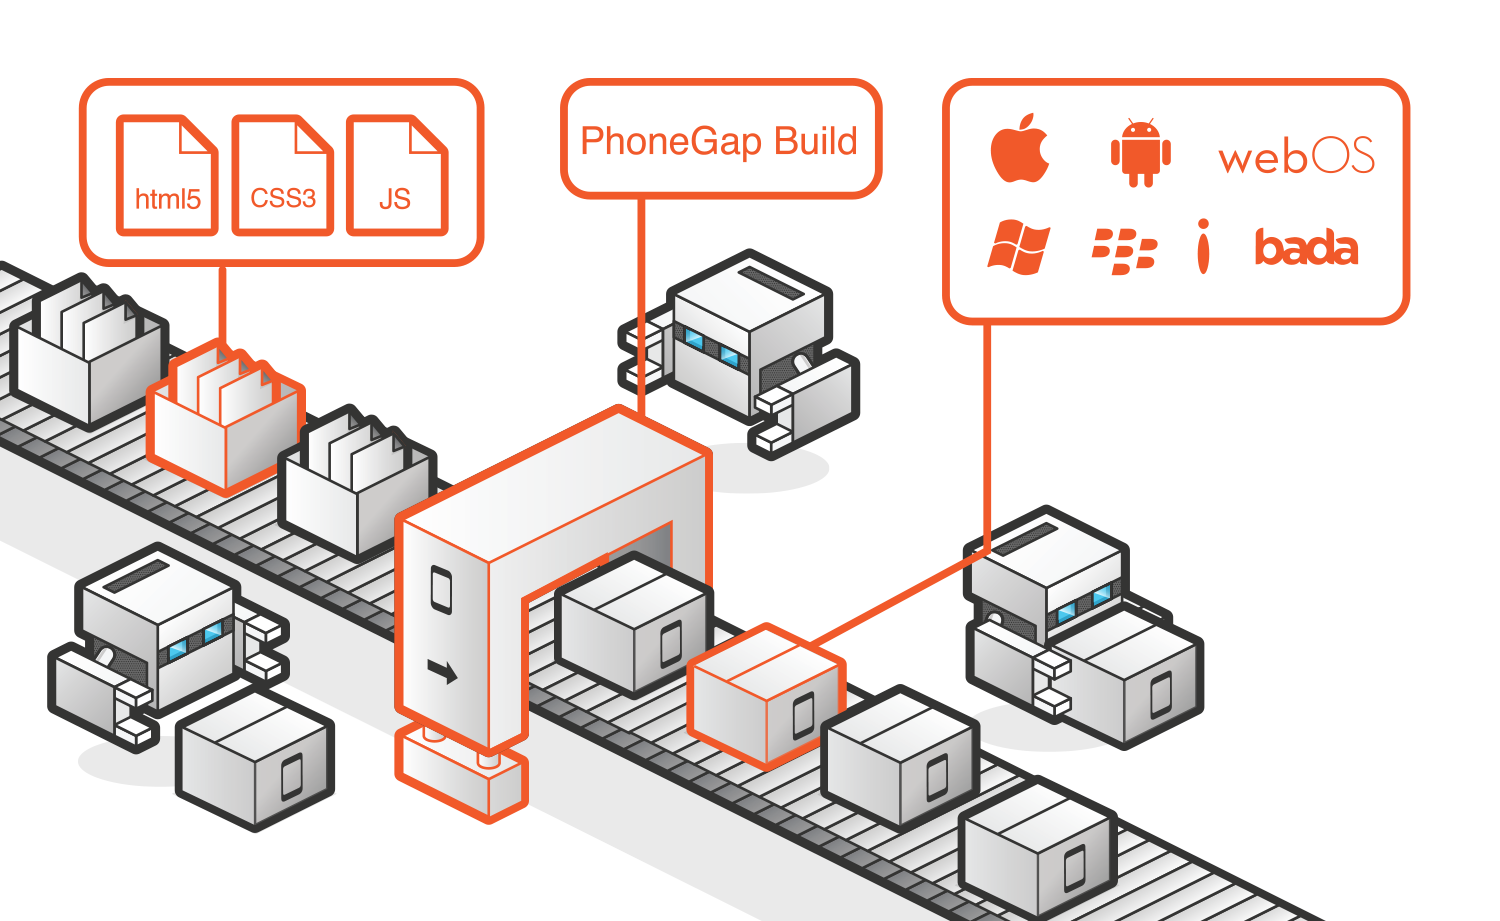
\includegraphics[width=14cm]{img/phonegap.png}
\label{Plateforme phonegap}
\end{center}


Lorsque vous utilisez l’API de PhoneGap, vous pouvez écrire votre application sans écrire de code natif (Java. Objectif-C, etc). Au lieu de cela, les technologies web sont utilisées, et sont hébérgées en local dans l’application elle même. Et parce que ces API JavaScript sont compatibles sur toutes les plateformes mobiles et construites sur les standards du Web, l’application doit être portable sur les plateformes des appareils avec peu ou pas de modifications.

PhoneGap enveloppe votre HTML et votre JavaScript avec juste assez de code natif pour que votre application web se sente plus à l’aise sur l’appareil. Cette enveloppe est différente pour chaque plateforme, mais elle expose ses capacités commune de manière cohérente. Cela vous permet d’écrire moins de code sur de multiples plateformes.

PhoneGap est disponible sur les plateformes suivantes: iOS, Android, Blackberry, Windows Phone, Palm WebOS, Bada et Symbian.

Depuis que PhoneGap enveloppe votre code HTML et JavaScript dans une application native, vous gagnez la possibilité de soumettre votre application au store de l’appareil. Chose que vous ne pouviez pas faire depuis une application web simple. Gardez à l’esprit, cependant, que la plupart des stores veulent que votre application ait le style d’une application native et que certains store sont plus strict que d’autres.

Voici une liste des composants supporté par PhoneGap.

\begin{center}
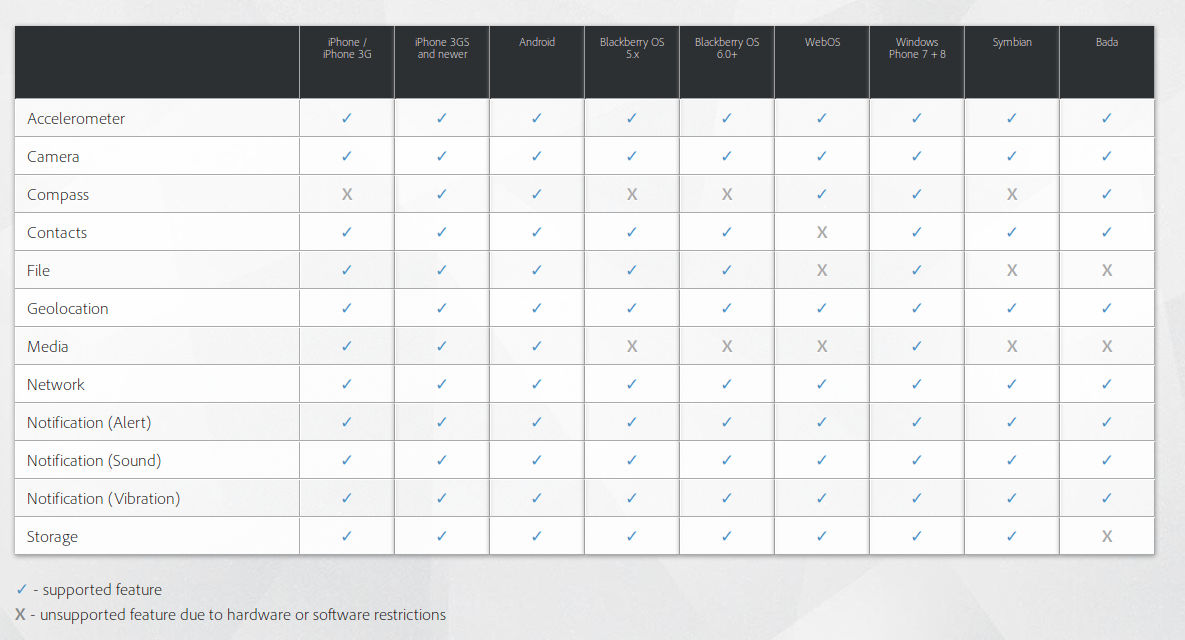
\includegraphics[width=14cm]{img/phonegapFeatures.png}
\label{Plateforme Wakanda}
\end{center}